\documentclass[]{article}
\usepackage{lmodern}
\usepackage{amssymb,amsmath}
\usepackage{ifxetex,ifluatex}
\usepackage{fixltx2e} % provides \textsubscript
\ifnum 0\ifxetex 1\fi\ifluatex 1\fi=0 % if pdftex
  \usepackage[T1]{fontenc}
  \usepackage[utf8]{inputenc}
\else % if luatex or xelatex
  \ifxetex
    \usepackage{mathspec}
  \else
    \usepackage{fontspec}
  \fi
  \defaultfontfeatures{Ligatures=TeX,Scale=MatchLowercase}
\fi
% use upquote if available, for straight quotes in verbatim environments
\IfFileExists{upquote.sty}{\usepackage{upquote}}{}
% use microtype if available
\IfFileExists{microtype.sty}{%
\usepackage{microtype}
\UseMicrotypeSet[protrusion]{basicmath} % disable protrusion for tt fonts
}{}
\usepackage[margin=1in]{geometry}
\usepackage{hyperref}
\hypersetup{unicode=true,
            pdftitle={Estatística Básica},
            pdfauthor={Luan Fiorentin},
            pdfborder={0 0 0},
            breaklinks=true}
\urlstyle{same}  % don't use monospace font for urls
\usepackage{color}
\usepackage{fancyvrb}
\newcommand{\VerbBar}{|}
\newcommand{\VERB}{\Verb[commandchars=\\\{\}]}
\DefineVerbatimEnvironment{Highlighting}{Verbatim}{commandchars=\\\{\}}
% Add ',fontsize=\small' for more characters per line
\usepackage{framed}
\definecolor{shadecolor}{RGB}{248,248,248}
\newenvironment{Shaded}{\begin{snugshade}}{\end{snugshade}}
\newcommand{\KeywordTok}[1]{\textcolor[rgb]{0.13,0.29,0.53}{\textbf{#1}}}
\newcommand{\DataTypeTok}[1]{\textcolor[rgb]{0.13,0.29,0.53}{#1}}
\newcommand{\DecValTok}[1]{\textcolor[rgb]{0.00,0.00,0.81}{#1}}
\newcommand{\BaseNTok}[1]{\textcolor[rgb]{0.00,0.00,0.81}{#1}}
\newcommand{\FloatTok}[1]{\textcolor[rgb]{0.00,0.00,0.81}{#1}}
\newcommand{\ConstantTok}[1]{\textcolor[rgb]{0.00,0.00,0.00}{#1}}
\newcommand{\CharTok}[1]{\textcolor[rgb]{0.31,0.60,0.02}{#1}}
\newcommand{\SpecialCharTok}[1]{\textcolor[rgb]{0.00,0.00,0.00}{#1}}
\newcommand{\StringTok}[1]{\textcolor[rgb]{0.31,0.60,0.02}{#1}}
\newcommand{\VerbatimStringTok}[1]{\textcolor[rgb]{0.31,0.60,0.02}{#1}}
\newcommand{\SpecialStringTok}[1]{\textcolor[rgb]{0.31,0.60,0.02}{#1}}
\newcommand{\ImportTok}[1]{#1}
\newcommand{\CommentTok}[1]{\textcolor[rgb]{0.56,0.35,0.01}{\textit{#1}}}
\newcommand{\DocumentationTok}[1]{\textcolor[rgb]{0.56,0.35,0.01}{\textbf{\textit{#1}}}}
\newcommand{\AnnotationTok}[1]{\textcolor[rgb]{0.56,0.35,0.01}{\textbf{\textit{#1}}}}
\newcommand{\CommentVarTok}[1]{\textcolor[rgb]{0.56,0.35,0.01}{\textbf{\textit{#1}}}}
\newcommand{\OtherTok}[1]{\textcolor[rgb]{0.56,0.35,0.01}{#1}}
\newcommand{\FunctionTok}[1]{\textcolor[rgb]{0.00,0.00,0.00}{#1}}
\newcommand{\VariableTok}[1]{\textcolor[rgb]{0.00,0.00,0.00}{#1}}
\newcommand{\ControlFlowTok}[1]{\textcolor[rgb]{0.13,0.29,0.53}{\textbf{#1}}}
\newcommand{\OperatorTok}[1]{\textcolor[rgb]{0.81,0.36,0.00}{\textbf{#1}}}
\newcommand{\BuiltInTok}[1]{#1}
\newcommand{\ExtensionTok}[1]{#1}
\newcommand{\PreprocessorTok}[1]{\textcolor[rgb]{0.56,0.35,0.01}{\textit{#1}}}
\newcommand{\AttributeTok}[1]{\textcolor[rgb]{0.77,0.63,0.00}{#1}}
\newcommand{\RegionMarkerTok}[1]{#1}
\newcommand{\InformationTok}[1]{\textcolor[rgb]{0.56,0.35,0.01}{\textbf{\textit{#1}}}}
\newcommand{\WarningTok}[1]{\textcolor[rgb]{0.56,0.35,0.01}{\textbf{\textit{#1}}}}
\newcommand{\AlertTok}[1]{\textcolor[rgb]{0.94,0.16,0.16}{#1}}
\newcommand{\ErrorTok}[1]{\textcolor[rgb]{0.64,0.00,0.00}{\textbf{#1}}}
\newcommand{\NormalTok}[1]{#1}
\usepackage{graphicx,grffile}
\makeatletter
\def\maxwidth{\ifdim\Gin@nat@width>\linewidth\linewidth\else\Gin@nat@width\fi}
\def\maxheight{\ifdim\Gin@nat@height>\textheight\textheight\else\Gin@nat@height\fi}
\makeatother
% Scale images if necessary, so that they will not overflow the page
% margins by default, and it is still possible to overwrite the defaults
% using explicit options in \includegraphics[width, height, ...]{}
\setkeys{Gin}{width=\maxwidth,height=\maxheight,keepaspectratio}
\IfFileExists{parskip.sty}{%
\usepackage{parskip}
}{% else
\setlength{\parindent}{0pt}
\setlength{\parskip}{6pt plus 2pt minus 1pt}
}
\setlength{\emergencystretch}{3em}  % prevent overfull lines
\providecommand{\tightlist}{%
  \setlength{\itemsep}{0pt}\setlength{\parskip}{0pt}}
\setcounter{secnumdepth}{0}
% Redefines (sub)paragraphs to behave more like sections
\ifx\paragraph\undefined\else
\let\oldparagraph\paragraph
\renewcommand{\paragraph}[1]{\oldparagraph{#1}\mbox{}}
\fi
\ifx\subparagraph\undefined\else
\let\oldsubparagraph\subparagraph
\renewcommand{\subparagraph}[1]{\oldsubparagraph{#1}\mbox{}}
\fi

%%% Use protect on footnotes to avoid problems with footnotes in titles
\let\rmarkdownfootnote\footnote%
\def\footnote{\protect\rmarkdownfootnote}

%%% Change title format to be more compact
\usepackage{titling}

% Create subtitle command for use in maketitle
\newcommand{\subtitle}[1]{
  \posttitle{
    \begin{center}\large#1\end{center}
    }
}

\setlength{\droptitle}{-2em}

  \title{Estatística Básica}
    \pretitle{\vspace{\droptitle}\centering\huge}
  \posttitle{\par}
  \subtitle{Lista 2 GABARITO - Medidas Resumo}
  \author{Luan Fiorentin}
    \preauthor{\centering\large\emph}
  \postauthor{\par}
      \predate{\centering\large\emph}
  \postdate{\par}
    \date{2019-03-05}

\usepackage{amsmath} \usepackage{float} \usepackage{bm}

\begin{document}
\maketitle

\begin{enumerate}
\def\labelenumi{\arabic{enumi}.}
\tightlist
\item
  Um exame de vestibular para uma faculdade tem 80 questões, sendo 40 de
  português e 40 de matemática. Para os 20 melhores classificados,
  apresentamos o número de acertos em cada disciplina, com os valores já
  ordenados.

  \begin{itemize}
  \tightlist
  \item
    Português: (8; 10; 11; 12; 12; 14; 17; 20; 20; 23; 23; 24; 26; 26;
    30; 31; 32; 34; 35; 35)
  \item
    Matemática: (13; 20; 20; 20; 21; 21; 23; 23; 25; 25; 26; 27; 28; 28;
    28; 29; 30; 31; 31; 32)
  \end{itemize}

  \begin{enumerate}
  \def\labelenumii{(\alph{enumii})}
  \tightlist
  \item
    Calcule as medidas de centro (média, mediana e moda) para cada
    grupo.
  \item
    Calcule as medidas de variabilidade (variância, desvio-padrão, e
    coeficiente de variação) para cada grupo.
  \item
    Calcule os quartis para cada grupo.
  \item
    Construa um gráfico de caixa (box plot) para cada grupo (em um mesmo
    gráfico para comparação).
  \item
    Com todos os resultados obtidos, descreva comparativamente os dois
    grupos em termos de medidas de tendência central, variabilidade,
    amplitude e distribuição (simetria) dos dados.
  \item
    Você acha que os aprovados são melhores em português ou matemática?
  \end{enumerate}
\end{enumerate}

\begin{Shaded}
\begin{Highlighting}[]
\CommentTok{# (a)}
\CommentTok{# Média}
\KeywordTok{mean}\NormalTok{(da1}\OperatorTok{$}\NormalTok{Por)}
\end{Highlighting}
\end{Shaded}

\begin{verbatim}
## [1] 22.15
\end{verbatim}

\begin{Shaded}
\begin{Highlighting}[]
\KeywordTok{mean}\NormalTok{(da1}\OperatorTok{$}\NormalTok{Mat)}
\end{Highlighting}
\end{Shaded}

\begin{verbatim}
## [1] 25.05
\end{verbatim}

\begin{Shaded}
\begin{Highlighting}[]
\CommentTok{# Mediana}
\KeywordTok{median}\NormalTok{(da1}\OperatorTok{$}\NormalTok{Por)}
\end{Highlighting}
\end{Shaded}

\begin{verbatim}
## [1] 23
\end{verbatim}

\begin{Shaded}
\begin{Highlighting}[]
\KeywordTok{median}\NormalTok{(da1}\OperatorTok{$}\NormalTok{Mat)}
\end{Highlighting}
\end{Shaded}

\begin{verbatim}
## [1] 25.5
\end{verbatim}

\begin{Shaded}
\begin{Highlighting}[]
\CommentTok{# Moda}
\CommentTok{# Para variável Português há 5 valores modais: 12; 20; 23; 26; 35.}
\CommentTok{# Para variável Matemática há 2 valores modais: 20; 28.}

\CommentTok{# (b)}
\CommentTok{# Variância}
\KeywordTok{var}\NormalTok{(da1}\OperatorTok{$}\NormalTok{Por)}
\end{Highlighting}
\end{Shaded}

\begin{verbatim}
## [1] 80.13421
\end{verbatim}

\begin{Shaded}
\begin{Highlighting}[]
\KeywordTok{var}\NormalTok{(da1}\OperatorTok{$}\NormalTok{Mat)}
\end{Highlighting}
\end{Shaded}

\begin{verbatim}
## [1] 23.83947
\end{verbatim}

\begin{Shaded}
\begin{Highlighting}[]
\CommentTok{# Desvio Padrão}
\KeywordTok{sd}\NormalTok{(da1}\OperatorTok{$}\NormalTok{Por)}
\end{Highlighting}
\end{Shaded}

\begin{verbatim}
## [1] 8.951771
\end{verbatim}

\begin{Shaded}
\begin{Highlighting}[]
\KeywordTok{sd}\NormalTok{(da1}\OperatorTok{$}\NormalTok{Mat)}
\end{Highlighting}
\end{Shaded}

\begin{verbatim}
## [1] 4.882568
\end{verbatim}

\begin{Shaded}
\begin{Highlighting}[]
\CommentTok{# Coeficiente de Variação}
\KeywordTok{coevar}\NormalTok{(da1}\OperatorTok{$}\NormalTok{Por)}
\end{Highlighting}
\end{Shaded}

\begin{verbatim}
## [1] 40.41432
\end{verbatim}

\begin{Shaded}
\begin{Highlighting}[]
\KeywordTok{coevar}\NormalTok{(da1}\OperatorTok{$}\NormalTok{Mat)}
\end{Highlighting}
\end{Shaded}

\begin{verbatim}
## [1] 19.49129
\end{verbatim}

\begin{Shaded}
\begin{Highlighting}[]
\CommentTok{# (c) Quantis}
\KeywordTok{quantile}\NormalTok{(da1}\OperatorTok{$}\NormalTok{Por)}
\end{Highlighting}
\end{Shaded}

\begin{verbatim}
##    0%   25%   50%   75%  100% 
##  8.00 13.50 23.00 30.25 35.00
\end{verbatim}

\begin{Shaded}
\begin{Highlighting}[]
\KeywordTok{quantile}\NormalTok{(da1}\OperatorTok{$}\NormalTok{Mat)}
\end{Highlighting}
\end{Shaded}

\begin{verbatim}
##    0%   25%   50%   75%  100% 
## 13.00 21.00 25.50 28.25 32.00
\end{verbatim}

\begin{Shaded}
\begin{Highlighting}[]
\CommentTok{# (d)}
\KeywordTok{boxplot}\NormalTok{(dab}\OperatorTok{$}\NormalTok{val }\OperatorTok{~}\StringTok{ }\NormalTok{dab}\OperatorTok{$}\NormalTok{var, }
        \DataTypeTok{ylim =} \KeywordTok{c}\NormalTok{(}\DecValTok{0}\NormalTok{,}\DecValTok{40}\NormalTok{), }
        \DataTypeTok{xlab =} \StringTok{"Disciplina"}\NormalTok{, }
        \DataTypeTok{ylab =} \StringTok{"Número de acertos"}\NormalTok{)}
\end{Highlighting}
\end{Shaded}

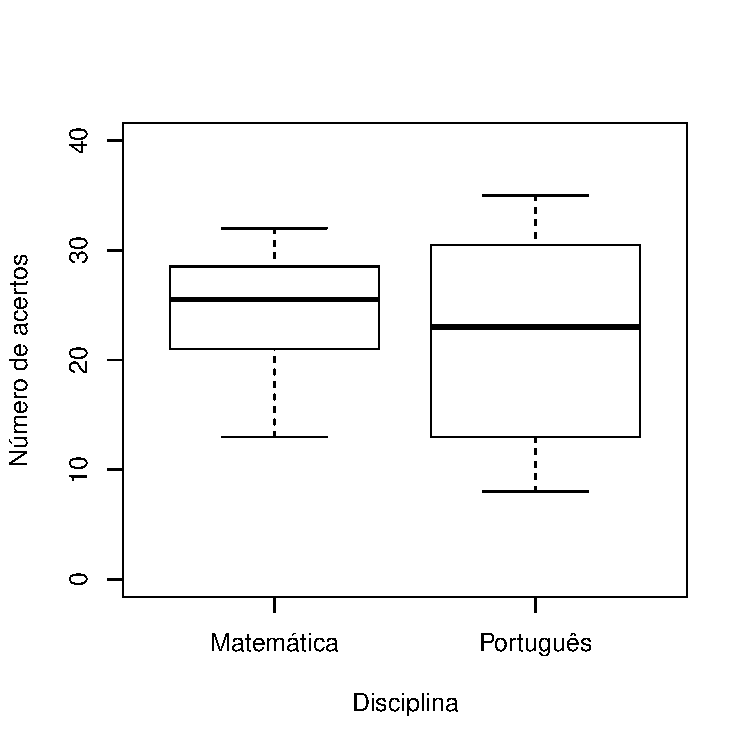
\includegraphics{Lista_2_Gabarito_files/figure-latex/unnamed-chunk-2-1.pdf}

\begin{Shaded}
\begin{Highlighting}[]
\CommentTok{# (e)}
\CommentTok{# Em média, o número de acertos em}
\CommentTok{# matemática (25,05) foi maior do que o número de}
\CommentTok{# acertos em português (22,15). A diferença entre}
\CommentTok{# os valores médios e a mediana mostra que existe uma leve assimetria}
\CommentTok{# negativa (ou à esquerda) para os dois casos (média < ,mediana),}
\CommentTok{# embora esta diferença seja mais evidente nas notas de}
\CommentTok{# português. A amplitude do número de acertos em português foi de}
\CommentTok{# 35-8=27, maior do que a amplitude obervada}
\CommentTok{# para o número de acertos em matemática, que foi de}
\CommentTok{# 32-13=19. A variabilidade dos acertos em torno}
\CommentTok{# da média também foi maior para as notas de português, com variância}
\CommentTok{# de 80,134 e desvio-padrão de 8,951. Já}
\CommentTok{# para a matemátiva, a variabilidade em torno da média foi menor, com}
\CommentTok{# 23,839 e desvio-padrão 4,883. Resumindo}
\CommentTok{# estas informações sobre variabilidade, nota-se que o coeficiente de}
\CommentTok{# variação para português foi de 40,4%, enquanto para a}
\CommentTok{# matemática foi menor, com aproximadamente 19,5%. Através do resumo}
\CommentTok{# dos cinco números e do gráfico de caixa, percebe-se que 50% dos}
\CommentTok{# acertos foram entre 13 e 30,5 em português (diferença entre Q1 e}
\CommentTok{# Q3), e entre 21 e 28,5 em matemática, mostrando novamente a menor}
\CommentTok{# variabilidade observada para a matemática.}
\end{Highlighting}
\end{Shaded}

\begin{enumerate}
\def\labelenumi{\arabic{enumi}.}
\setcounter{enumi}{1}
\tightlist
\item
  Considere a amostras de alturas de uma espécie de árvore (metros),
  coletadas em quatro áreas diferentes.

  \begin{itemize}
  \tightlist
  \item
    Área A: (9,2; 10,8; 10,6; 11,1; 12,1; 9,6; 11,2; 8,4; 12,9; 12,1;
    14,4; 11,1; 11,1; 9,7; 8,4; 12,3; 10,7; 12,9; 9,1; 12,8).
  \item
    Área B: (12,5; 18,5; 21,3; 14,3; 18,5; 19,0; 10,8; 23,1; 17,4; 10,7;
    14,3; 16,3; 18,0; 7,1; 12,8; 14,7; 11,3; 8,2; 13,8).
  \item
    Área C: (21,3; 28,7; 15,8; 24,0; 13,7; 18,1; 12,6; 14,6; 6,1; 19,8;
    22,3; 15,7; 16,3; 18,2; 15,7; 6,6; 9,3; 1,3; 19,0).
  \item
    Área D: (13,7; 8,6; 14,9; 10,2; 14,0; 10,5; 15,0; 5,2; 10,0; 11,7;
    18,7; 9,3; 7,9; 6,5; 11,5; 12,0; 8,3; 8,3; 9,8; 4,7).
  \end{itemize}

  \begin{enumerate}
  \def\labelenumii{(\alph{enumii})}
  \tightlist
  \item
    Calcule as medidas de amplitude, média, mediana, variância, desvio
    padrão e coeficiente de variação para as quatro áreas.
  \item
    Descreva comparativamente as quatro áreas quanto à altura das
    árvores, utilizando as estatísticas que você calculou.
  \end{enumerate}
\end{enumerate}

\begin{Shaded}
\begin{Highlighting}[]
\CommentTok{# (a) Estatísticas calculadas}
\KeywordTok{round}\NormalTok{(}\KeywordTok{apply}\NormalTok{(da2, }\DecValTok{2}\NormalTok{, estat_descritiva), }\DecValTok{3}\NormalTok{)}
\end{Highlighting}
\end{Shaded}

\begin{verbatim}
##                AreaA  AreaB  AreaC  AreaD
## Mínimo         8.400  7.100  1.300  4.700
## Média         11.025 14.665 15.805 10.540
## Mediana       11.100 14.300 16.050 10.100
## Máximo        14.400 23.100 28.700 18.700
## Amplitude      6.000 16.000 27.400 14.000
## Variância      2.658 18.451 41.709 12.318
## Desvio Padrão  1.630  4.295  6.458  3.510
## CV            14.787 29.290 40.862 33.299
\end{verbatim}

\begin{Shaded}
\begin{Highlighting}[]
\CommentTok{# (b)}
\CommentTok{# Em média, a área C possui as árvores}
\CommentTok{# mais altas (18,8), enquanto a área D possui as}
\CommentTok{# árvores mais baixas (10,5). Em todas as áreas, o valor}
\CommentTok{# da mediana está muito próximo do valor da média, o que}
\CommentTok{# indica que a distribuição das alturas em todas as áreas é}
\CommentTok{# aproximadamente simétrica. A maior amplitude de variação de alturas}
\CommentTok{# foi observada na área C, que também apresentou a maior variabilidade}
\CommentTok{# das observações em relação à média, como pode ser observado pelos}
\CommentTok{# valores da variância (43,943), e do desvio-padrão (6,629). }
\CommentTok{# A área com árvores de alturas mais homogêneas foi a A, pois a}
\CommentTok{# amplitude foi de 6 m, e a varibilidade das alturas em torno da média}
\CommentTok{# foi a menor quando comparada com as demais áreas (A = 2,66 e}
\CommentTok{# 1,63). Estas diferenças de variabilidade podem ser observadas}
\CommentTok{# através do coeficiente de variação, que foi de 40,9% para a área C, e}
\CommentTok{# de 14,8% para a área A. A área D apresentou um CV de 33,3%, enquanto}
\CommentTok{# o CV da área B foi de 29,3%.}
\end{Highlighting}
\end{Shaded}

\begin{enumerate}
\def\labelenumi{\arabic{enumi}.}
\setcounter{enumi}{2}
\tightlist
\item
  Deseja-se comparar três métodos de ensino no aprendizado de
  estatística. Cada método foi aplicado a 30 alunos e os resultados
  estão apresentados nos boxplot abaixo.

  \begin{enumerate}
  \def\labelenumii{(\alph{enumii})}
  \tightlist
  \item
    Encontre os valores (aproximados) para a mediana, os quartis, máximo
    e mínimo.
  \item
    Discuta a variabilidade do tempo de aprendizado de cada método.
  \item
    Se você é otimista, qual método escolheria?
  \end{enumerate}
\end{enumerate}

\begin{figure}[H]
\centering
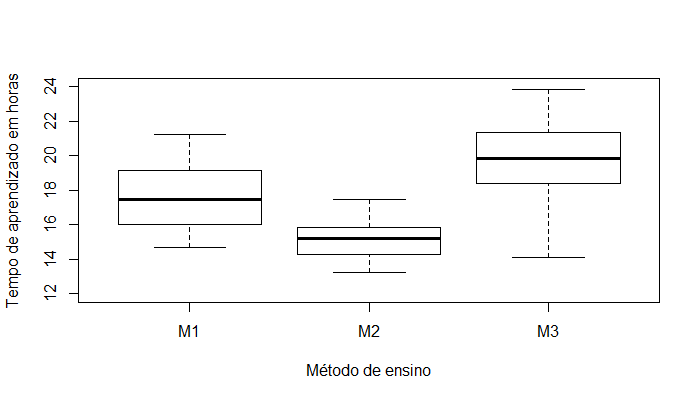
\includegraphics[]{ex3.PNG}
\end{figure}

\begin{Shaded}
\begin{Highlighting}[]
\CommentTok{# (a)}
\CommentTok{# Observação: São valores verdadeiros.}
\KeywordTok{round}\NormalTok{(}\KeywordTok{apply}\NormalTok{(daresul, }\DecValTok{2}\NormalTok{, quantile), }\DecValTok{3}\NormalTok{)}
\end{Highlighting}
\end{Shaded}

\begin{verbatim}
##          M1     M2     M3
## 0%   14.675 13.219 14.114
## 25%  16.087 14.302 18.507
## 50%  17.499 15.227 19.872
## 75%  19.136 15.841 21.219
## 100% 21.225 17.473 23.869
\end{verbatim}

\begin{Shaded}
\begin{Highlighting}[]
\CommentTok{#(b)}
\CommentTok{# A amplitude do tempo de aprendizado para}
\CommentTok{# os métodos M1, M2 e M3 são: M1 = 6,550, M2 = 4,254, e M3 = 9,755. }
\CommentTok{# Com isso, percebe-se que:}
\CommentTok{# o método M1 apresenta um tempo aprendizado (aproximado) entre 14 e 21}
\CommentTok{# horas, o método M2 entre 13 e 17 horas, e o método M3 entre 14 e 23}
\CommentTok{# horas. A maior variação de tempo de recuperação foi então do método M3}
\CommentTok{# (maior amplitude), enquanto o método M2 apresentou a menor}
\CommentTok{# variação. Nota-se, em termos de mediana, que o método M2 apresentou o}
\CommentTok{# menor tempo de aprendizado (Me = 15,227), e com uma pequena}
\CommentTok{# variabilidade. Além disso, percebe-se através do gráfico boxplot, que}
\CommentTok{# os métodos M1 e M3 possuem uma distribuição simétrica, como pode}
\CommentTok{# ser observado pela proximidade da mediana com o primeiro (Q1) e terceiro quartil}
\CommentTok{# (Q3). Percebe-se também que a distribuição do tempo de aprendizado do método M2}
\CommentTok{# é levemente assimétrica à direita, pois a mediana está deslocada para cima}
\CommentTok{# dentro da caixa. O tempo de de aprendizado mediano para o método M2 foi}
\CommentTok{# de 15,227. Para esse método, 50\textbackslash{}% das pessoas tiveram um tempo de}
\CommentTok{# recuperação entre 14,302 (Q1) e 15,841 (Q3) horas.}
\end{Highlighting}
\end{Shaded}

\begin{enumerate}
\def\labelenumi{\arabic{enumi}.}
\setcounter{enumi}{3}
\tightlist
\item
  A distribuição das estaturas, em centímetros, de alunos de um curso
  colegial está representada na tabela de frequência abaixo. Calcule a
  média, a variância, e o desvio-padrão das estaturas.
\end{enumerate}

\begin{table}[H]
\centering
\begin{tabular}{cc}
\hline
Classes     & Frequência \\ \hline
{[}135-145) & 15         \\
{[}145-155) & 150        \\
{[}155-165) & 250        \\
{[}165-175) & 70         \\
{[}175-185) & 10         \\
{[}185-195] & 5          \\ \hline
\end{tabular}
\end{table}

\begin{Shaded}
\begin{Highlighting}[]
\CommentTok{# Tabela auxiliar}
\KeywordTok{data.frame}\NormalTok{(xi, fi, xifi, xi2, xi2fi)}
\end{Highlighting}
\end{Shaded}

\begin{verbatim}
##    xi  fi  xifi   xi2   xi2fi
## 1 140  15  2100 19600  294000
## 2 150 150 22500 22500 3375000
## 3 160 250 40000 25600 6400000
## 4 170  70 11900 28900 2023000
## 5 180  10  1800 32400  324000
## 6 190   5   950 36100  180500
\end{verbatim}

\begin{Shaded}
\begin{Highlighting}[]
\CommentTok{# Média}
\KeywordTok{sum}\NormalTok{(xifi }\OperatorTok{/}\StringTok{ }\KeywordTok{sum}\NormalTok{(fi))}
\end{Highlighting}
\end{Shaded}

\begin{verbatim}
## [1] 158.5
\end{verbatim}

\begin{Shaded}
\begin{Highlighting}[]
\CommentTok{# Variância}
\NormalTok{(}\DecValTok{1}\OperatorTok{/}\NormalTok{(}\KeywordTok{sum}\NormalTok{(fi)}\OperatorTok{-}\DecValTok{1}\NormalTok{)) }\OperatorTok{*}\StringTok{ }\NormalTok{(}\KeywordTok{sum}\NormalTok{(xi2fi) }\OperatorTok{-}\StringTok{ }\KeywordTok{sum}\NormalTok{(xifi)}\OperatorTok{^}\DecValTok{2}\OperatorTok{/}\KeywordTok{sum}\NormalTok{(fi))}
\end{Highlighting}
\end{Shaded}

\begin{verbatim}
## [1] 70.89178
\end{verbatim}

\begin{Shaded}
\begin{Highlighting}[]
\CommentTok{# Desvio Padrão}
\KeywordTok{sqrt}\NormalTok{((}\DecValTok{1}\OperatorTok{/}\NormalTok{(}\KeywordTok{sum}\NormalTok{(fi)}\OperatorTok{-}\DecValTok{1}\NormalTok{)) }\OperatorTok{*}\StringTok{ }\NormalTok{(}\KeywordTok{sum}\NormalTok{(xi2fi) }\OperatorTok{-}\StringTok{ }\KeywordTok{sum}\NormalTok{(xifi)}\OperatorTok{^}\DecValTok{2}\OperatorTok{/}\KeywordTok{sum}\NormalTok{(fi)))}
\end{Highlighting}
\end{Shaded}

\begin{verbatim}
## [1] 8.419726
\end{verbatim}

\begin{enumerate}
\def\labelenumi{\arabic{enumi}.}
\setcounter{enumi}{4}
\tightlist
\item
  Os dados abaixo representam as vendas semanais, em classes de salários
  mínimos, de vendedores de gêneros alimentícios:

  \begin{enumerate}
  \def\labelenumii{(\alph{enumii})}
  \tightlist
  \item
    Faça o histograma das observações.
  \item
    Calcule a média da amostra (\(\bar x\)).
  \item
    Calcule o desvio-padrão da amostra.
  \item
    Calcule o primeiro quartil (\(Q_1\)), mediana (\(Q_2\)) e o terceiro
    quartil (\(Q_3\)).
  \end{enumerate}
\end{enumerate}

\begin{table}[H]
\centering
\begin{tabular}{cc}
\hline
Vendas    & Vendedores \\ \hline
{[}30-35) & 2          \\
{[}35-40) & 10         \\
{[}40-45) & 18         \\
{[}45-50) & 50         \\
{[}50-55) & 70         \\
{[}55-60) & 30         \\
{[}60-65) & 18         \\
{[}65-70) & 2          \\ \hline
\end{tabular}
\end{table}

\begin{Shaded}
\begin{Highlighting}[]
\CommentTok{# (a)}
\KeywordTok{barplot}\NormalTok{(fi, }
        \DataTypeTok{space =} \DecValTok{0}\NormalTok{, }
        \DataTypeTok{names.arg =}\NormalTok{ xi, }
        \DataTypeTok{xlab =} \StringTok{"Ponto médio"}\NormalTok{, }
        \DataTypeTok{ylab =} \StringTok{"Frequência", }
\StringTok{        col = "}\NormalTok{white}\StringTok{")}
\end{Highlighting}
\end{Shaded}

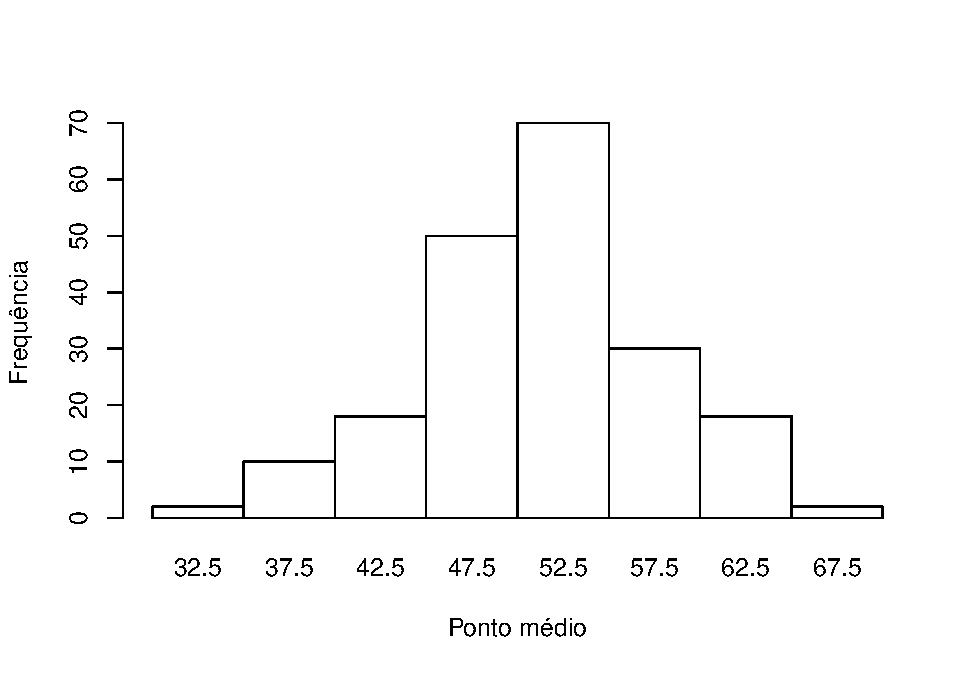
\includegraphics{Lista_2_Gabarito_files/figure-latex/unnamed-chunk-10-1.pdf}

\begin{Shaded}
\begin{Highlighting}[]
\CommentTok{# Tabela auxiliar}
\KeywordTok{data.frame}\NormalTok{(xi, fi, xifi, xi2, xi2fi)}
\end{Highlighting}
\end{Shaded}

\begin{verbatim}
##     xi fi xifi     xi2    xi2fi
## 1 32.5  2   65 1056.25   2112.5
## 2 37.5 10  375 1406.25  14062.5
## 3 42.5 18  765 1806.25  32512.5
## 4 47.5 50 2375 2256.25 112812.5
## 5 52.5 70 3675 2756.25 192937.5
## 6 57.5 30 1725 3306.25  99187.5
## 7 62.5 18 1125 3906.25  70312.5
## 8 67.5  2  135 4556.25   9112.5
\end{verbatim}

\begin{Shaded}
\begin{Highlighting}[]
\CommentTok{# (b)}
\CommentTok{# Média}
\KeywordTok{sum}\NormalTok{(xifi }\OperatorTok{/}\StringTok{ }\KeywordTok{sum}\NormalTok{(fi))}
\end{Highlighting}
\end{Shaded}

\begin{verbatim}
## [1] 51.2
\end{verbatim}

\begin{Shaded}
\begin{Highlighting}[]
\CommentTok{# (c)}
\CommentTok{# Variância}
\NormalTok{(}\DecValTok{1}\OperatorTok{/}\NormalTok{(}\KeywordTok{sum}\NormalTok{(fi)}\OperatorTok{-}\DecValTok{1}\NormalTok{)) }\OperatorTok{*}\StringTok{ }\NormalTok{(}\KeywordTok{sum}\NormalTok{(xi2fi) }\OperatorTok{-}\StringTok{ }\KeywordTok{sum}\NormalTok{(xifi)}\OperatorTok{^}\DecValTok{2}\OperatorTok{/}\KeywordTok{sum}\NormalTok{(fi))}
\end{Highlighting}
\end{Shaded}

\begin{verbatim}
## [1] 44.03015
\end{verbatim}

\begin{Shaded}
\begin{Highlighting}[]
\CommentTok{# Desvio Padrão}
\KeywordTok{sqrt}\NormalTok{((}\DecValTok{1}\OperatorTok{/}\NormalTok{(}\KeywordTok{sum}\NormalTok{(fi)}\OperatorTok{-}\DecValTok{1}\NormalTok{)) }\OperatorTok{*}\StringTok{ }\NormalTok{(}\KeywordTok{sum}\NormalTok{(xi2fi) }\OperatorTok{-}\StringTok{ }\KeywordTok{sum}\NormalTok{(xifi)}\OperatorTok{^}\DecValTok{2}\OperatorTok{/}\KeywordTok{sum}\NormalTok{(fi)))}
\end{Highlighting}
\end{Shaded}

\begin{verbatim}
## [1] 6.635522
\end{verbatim}

\begin{Shaded}
\begin{Highlighting}[]
\CommentTok{# (d)}
\KeywordTok{cumsum}\NormalTok{(}\KeywordTok{prop.table}\NormalTok{(fi))}
\end{Highlighting}
\end{Shaded}

\begin{verbatim}
## [1] 0.01 0.06 0.15 0.40 0.75 0.90 0.99 1.00
\end{verbatim}

\begin{Shaded}
\begin{Highlighting}[]
\CommentTok{# Considerando que}
\CommentTok{# (55-50)/0,35 = (Q2-50)/0,10}
\CommentTok{# Então a mediana é}
\NormalTok{(Q2 <-}\StringTok{ }\NormalTok{((}\DecValTok{55}\OperatorTok{-}\DecValTok{50}\NormalTok{)}\OperatorTok{/}\FloatTok{0.35}\NormalTok{) }\OperatorTok{*}\StringTok{ }\FloatTok{0.10} \OperatorTok{+}\StringTok{ }\DecValTok{50}\NormalTok{)}
\end{Highlighting}
\end{Shaded}

\begin{verbatim}
## [1] 51.42857
\end{verbatim}

\begin{Shaded}
\begin{Highlighting}[]
\NormalTok{(Q1 <-}\StringTok{ }\NormalTok{((}\DecValTok{50}\OperatorTok{-}\DecValTok{45}\NormalTok{)}\OperatorTok{/}\FloatTok{0.25}\NormalTok{) }\OperatorTok{*}\StringTok{ }\FloatTok{0.10} \OperatorTok{+}\StringTok{ }\DecValTok{45}\NormalTok{)}
\end{Highlighting}
\end{Shaded}

\begin{verbatim}
## [1] 47
\end{verbatim}

\begin{Shaded}
\begin{Highlighting}[]
\NormalTok{(Q3 <-}\StringTok{ }\NormalTok{((}\DecValTok{55}\OperatorTok{-}\DecValTok{50}\NormalTok{)}\OperatorTok{/}\FloatTok{0.35}\NormalTok{) }\OperatorTok{*}\StringTok{ }\FloatTok{0.35} \OperatorTok{+}\StringTok{ }\DecValTok{50}\NormalTok{)}
\end{Highlighting}
\end{Shaded}

\begin{verbatim}
## [1] 55
\end{verbatim}

\begin{enumerate}
\def\labelenumi{\arabic{enumi}.}
\setcounter{enumi}{5}
\tightlist
\item
  O departamento pessoal de uma certa firma fez um levantamento dos
  salários dos 120 funcionários do setor administrativo, obtendo os
  resultados (em salários mínimos) da tabela abaixo.

  \begin{enumerate}
  \def\labelenumii{(\alph{enumii})}
  \tightlist
  \item
    Calcule a média, a mediana, a variância e o desvio-padrão
  \item
    Se for concedido um aumento de 100\% para todos os 120 funcionários,
    haverá alteração na média? E na variância? Justifique sua resposta.
  \item
    Se for concedido um abono de dois salários mínimos para todos os 120
    funcionários, haverá alteração na média? E na mediana? E na
    variância? Justifique sua resposta.
  \end{enumerate}
\end{enumerate}

\begin{table}[H]
\centering
\begin{tabular}{ll}
\hline
Salários   & Freq. relativa \\ \hline
{[}0-2)    & 0,25           \\
{[}2-4)    & 0,40           \\
{[}4-6)    & 0,20           \\
{[}6-10{]} & 0,15           \\ \hline
\end{tabular}
\end{table}

\begin{Shaded}
\begin{Highlighting}[]
\CommentTok{# (a)}
\CommentTok{# Tabela auxiliar}
\KeywordTok{data.frame}\NormalTok{(xi, fi, xifi, xi2, xi2fi)}
\end{Highlighting}
\end{Shaded}

\begin{verbatim}
##   xi fi xifi xi2 xi2fi
## 1  1 30   30   1    30
## 2  3 48  144   9   432
## 3  5 24  120  25   600
## 4  8 18  144  64  1152
\end{verbatim}

\begin{Shaded}
\begin{Highlighting}[]
\CommentTok{# Média}
\KeywordTok{sum}\NormalTok{(xifi }\OperatorTok{/}\StringTok{ }\KeywordTok{sum}\NormalTok{(fi))}
\end{Highlighting}
\end{Shaded}

\begin{verbatim}
## [1] 3.65
\end{verbatim}

\begin{Shaded}
\begin{Highlighting}[]
\CommentTok{# Variância}
\NormalTok{(}\DecValTok{1}\OperatorTok{/}\NormalTok{(}\DecValTok{120}\NormalTok{)) }\OperatorTok{*}\StringTok{ }\NormalTok{(}\KeywordTok{sum}\NormalTok{(xi2fi) }\OperatorTok{-}\StringTok{ }\NormalTok{(}\KeywordTok{sum}\NormalTok{(xifi)}\OperatorTok{^}\DecValTok{2}\NormalTok{)}\OperatorTok{/}\DecValTok{120}\NormalTok{)}
\end{Highlighting}
\end{Shaded}

\begin{verbatim}
## [1] 5.1275
\end{verbatim}

\begin{Shaded}
\begin{Highlighting}[]
\CommentTok{# Desvio Padrão}
\KeywordTok{sqrt}\NormalTok{((}\DecValTok{1}\OperatorTok{/}\NormalTok{(}\DecValTok{120}\NormalTok{)) }\OperatorTok{*}\StringTok{ }\NormalTok{(}\KeywordTok{sum}\NormalTok{(xi2fi) }\OperatorTok{-}\StringTok{ }\NormalTok{(}\KeywordTok{sum}\NormalTok{(xifi)}\OperatorTok{^}\DecValTok{2}\NormalTok{)}\OperatorTok{/}\DecValTok{120}\NormalTok{))}
\end{Highlighting}
\end{Shaded}

\begin{verbatim}
## [1] 2.264398
\end{verbatim}

\begin{Shaded}
\begin{Highlighting}[]
\CommentTok{# Mediana}
\NormalTok{(Q2 <-}\StringTok{ }\NormalTok{((}\DecValTok{4}\OperatorTok{-}\DecValTok{2}\NormalTok{)}\OperatorTok{/}\FloatTok{0.40}\NormalTok{) }\OperatorTok{*}\StringTok{ }\FloatTok{0.25} \OperatorTok{+}\StringTok{ }\DecValTok{2}\NormalTok{)}
\end{Highlighting}
\end{Shaded}

\begin{verbatim}
## [1] 3.25
\end{verbatim}

\begin{Shaded}
\begin{Highlighting}[]
\CommentTok{# (b)}
\CommentTok{# Haverá alteração na média, pois é multiplicada por 2}
\KeywordTok{sum}\NormalTok{(xifi }\OperatorTok{/}\StringTok{ }\KeywordTok{sum}\NormalTok{(fi)) }\OperatorTok{*}\StringTok{ }\DecValTok{2}
\end{Highlighting}
\end{Shaded}

\begin{verbatim}
## [1] 7.3
\end{verbatim}

\begin{Shaded}
\begin{Highlighting}[]
\CommentTok{# Haverá alteração na variância, pois é multiplicada por 4}
\NormalTok{(}\DecValTok{1}\OperatorTok{/}\NormalTok{(}\DecValTok{120}\NormalTok{)) }\OperatorTok{*}\StringTok{ }\NormalTok{(}\KeywordTok{sum}\NormalTok{(xi2fi) }\OperatorTok{-}\StringTok{ }\NormalTok{(}\KeywordTok{sum}\NormalTok{(xifi)}\OperatorTok{^}\DecValTok{2}\NormalTok{)}\OperatorTok{/}\DecValTok{120}\NormalTok{) }\OperatorTok{*}\StringTok{ }\DecValTok{4}
\end{Highlighting}
\end{Shaded}

\begin{verbatim}
## [1] 20.51
\end{verbatim}

\begin{Shaded}
\begin{Highlighting}[]
\CommentTok{#(c)}
\CommentTok{# Haverá alteração na média, pois é somada em 2 unidades}
\KeywordTok{sum}\NormalTok{(xifi }\OperatorTok{/}\StringTok{ }\KeywordTok{sum}\NormalTok{(fi)) }\OperatorTok{+}\StringTok{ }\DecValTok{2}
\end{Highlighting}
\end{Shaded}

\begin{verbatim}
## [1] 5.65
\end{verbatim}

\begin{Shaded}
\begin{Highlighting}[]
\CommentTok{# Haverá alteração na mediana, pois é somada em 2 unidades}
\NormalTok{(Q2 <-}\StringTok{ }\NormalTok{(((}\DecValTok{4}\OperatorTok{-}\DecValTok{2}\NormalTok{)}\OperatorTok{/}\FloatTok{0.40}\NormalTok{) }\OperatorTok{*}\StringTok{ }\FloatTok{0.25} \OperatorTok{+}\StringTok{ }\DecValTok{2}\NormalTok{) }\OperatorTok{+}\StringTok{ }\DecValTok{2}\NormalTok{)}
\end{Highlighting}
\end{Shaded}

\begin{verbatim}
## [1] 5.25
\end{verbatim}

\begin{Shaded}
\begin{Highlighting}[]
\CommentTok{# Não haverá mudança na variância, pois apenas acrescentou-se um}
\CommentTok{# um valor constante}
\NormalTok{(}\DecValTok{1}\OperatorTok{/}\NormalTok{(}\DecValTok{120}\NormalTok{)) }\OperatorTok{*}\StringTok{ }\NormalTok{(}\KeywordTok{sum}\NormalTok{(xi2fi) }\OperatorTok{-}\StringTok{ }\NormalTok{(}\KeywordTok{sum}\NormalTok{(xifi)}\OperatorTok{^}\DecValTok{2}\NormalTok{)}\OperatorTok{/}\DecValTok{120}\NormalTok{)}
\end{Highlighting}
\end{Shaded}

\begin{verbatim}
## [1] 5.1275
\end{verbatim}

\begin{enumerate}
\def\labelenumi{\arabic{enumi}.}
\setcounter{enumi}{6}
\tightlist
\item
  O resultado de uma prova de estatística aplicada à 25 alunos foi o
  seguinte:
\end{enumerate}

\[(9, 9, 8, 8, 9, 10, 8, 8, 9, 8, 10, 7, 7, 9, 9, 7, 8, 9, 4, 7, 7, 8, 10, 9, 9)\]

Como os alunos possuiam diferentes níveis educacionais, decidiu-se
calcular o desempenho relativo de cada candidato, para facilitar a
interpretação dos resultados. Essa medida de desempenho relativo será
obtida da seguinte forma: 1. Calcula-se a média (\(\bar x\)) e o
desvio-padrão (\(s\)) da amostra. 2. A nota \(x_i\) de cada aluno será
padronizada da seguinte forma:

\[z_i = \frac{x_i - \bar x}{s}.\]

Assim, criou-se uma nova variável \(Z\) que corresponde ao conjunto de
notas padronizadas. Com isso:

\begin{enumerate}
\def\labelenumi{(\alph{enumi})}
\tightlist
\item
  Calcule as notas padronizadas de todos os funcionários.
\item
  Com os resultados obtidos acima, calcule a média (\(\bar z\)) e o
  desvio-padrão (\(s_z\)) de \(Z\).
\item
  Se alguma das notas padronizadas estiver acima de \(2s_z\) ou abaixo
  de \(-2s_z\), esse aluno deve ser considerado ``atípico''. Existe
  algum nessa situação?
\item
  Interprete o significado de \(Z\).
\end{enumerate}

\begin{Shaded}
\begin{Highlighting}[]
\CommentTok{# (a)}
\CommentTok{# Média}
\KeywordTok{mean}\NormalTok{(da7)}
\end{Highlighting}
\end{Shaded}

\begin{verbatim}
## [1] 8.24
\end{verbatim}

\begin{Shaded}
\begin{Highlighting}[]
\CommentTok{# Variância}
\KeywordTok{sd}\NormalTok{(da7)}
\end{Highlighting}
\end{Shaded}

\begin{verbatim}
## [1] 1.3
\end{verbatim}

\begin{Shaded}
\begin{Highlighting}[]
\CommentTok{# Padronizando}
\NormalTok{(xi_pad <-}\StringTok{ }\NormalTok{(da7 }\OperatorTok{-}\StringTok{ }\KeywordTok{mean}\NormalTok{(da7)) }\OperatorTok{/}\StringTok{ }\KeywordTok{sd}\NormalTok{(da7))}
\end{Highlighting}
\end{Shaded}

\begin{verbatim}
##  [1]  0.5846154  0.5846154 -0.1846154 -0.1846154  0.5846154  1.3538462
##  [7] -0.1846154 -0.1846154  0.5846154 -0.1846154  1.3538462 -0.9538462
## [13] -0.9538462  0.5846154  0.5846154 -0.9538462 -0.1846154  0.5846154
## [19] -3.2615385 -0.9538462 -0.9538462 -0.1846154  1.3538462  0.5846154
## [25]  0.5846154
\end{verbatim}

\begin{Shaded}
\begin{Highlighting}[]
\CommentTok{# (b)}
\CommentTok{# Média}
\KeywordTok{mean}\NormalTok{(xi_pad)}
\end{Highlighting}
\end{Shaded}

\begin{verbatim}
## [1] -1.587923e-16
\end{verbatim}

\begin{Shaded}
\begin{Highlighting}[]
\CommentTok{# Desvio Padrão}
\KeywordTok{sd}\NormalTok{(xi_pad)}
\end{Highlighting}
\end{Shaded}

\begin{verbatim}
## [1] 1
\end{verbatim}

\begin{Shaded}
\begin{Highlighting}[]
\CommentTok{# (c)}
\CommentTok{# Sim, o valor atípico é -3,33,}
\CommentTok{# e corresponde a nota 4.}

\CommentTok{# (d)}
\CommentTok{# A variável Z é uma variável padronizada, que mede o número de desvios padrões}
\CommentTok{# que cada observação se afasta de média.}
\end{Highlighting}
\end{Shaded}


\end{document}
